%% notes-tex/multimodal/043-datasets-primer/sections/output-design.tex
%% SOURCE: the numbers are read from notes/experiments.043-expression-proteome-morphology.md
%% (cross_dataset_correlation.py, jobs 5890 and 5892; within_dataset_ceilings.py, jobs 5893,
%% 5895, 5896, 5898; store_census.py), from the 019 campaign write-up on the
%% multimodal-phenotype-retrospective worktree (notes-tex/figure-3-gate/sections/10-data-review.tex
%% and 11-inductive.tex; notes-tex/019-simb-multimodal-expression/sections/2-readouts.tex), from
%% the 035 note (notes/experiments.035-env-chemgen-vanacloig-cgt.md, rounds 9 and 10) and from
%% the Sameith 2015 paper in the mirror (sameithHighresolutionGeneExpression2015/paper.md).
%% The prototype of the heads and the loss is torchcell/models/readout_heads_043.py, tested by
%% tests/torchcell/models/test_readout_heads_043.py; the diagram is
%% notes/experiments.043-expression-proteome-morphology.mermaid.output-side.md.

\section{The output side: readouts, heads, tokens, losses and the evaluation\secstatus{todo}}
\label{sec:output}

What follows is a design for the group to accept, change or reject. The owner's direction
fixes three things: every gene-level readout is trained on; a readout is read off the
perturbed graph, ``from the node itself'' for a gene-level value; and the question to
answer is whether the model improves on held-out Kemmeren single deletions and on the
Sameith double deletions, with Muenzner 2024 as a proteome test and Ohya 2005 CalMorph as a
probe of the learned state and never a training target. Everything else below is a choice
with its facts, Fig.~\ref{fig:output-side} draws the path, and
Sec.~\ref{sec:output-decisions} lists the choices the owner has to make.

%% SOURCE: hand-authored definitions; the numbers in cells cite their section.
\begin{table}[htbp]
\centering
\footnotesize
\caption[]{\textbf{Terms of this section}, alphabetical. Terms of Table~\ref{tab:vocab}
are not repeated.}
\label{tab:output-vocab}
\begin{tabular}{>{\raggedright\arraybackslash}p{30mm}>{\raggedright\arraybackslash}p{140mm}}
\toprule
Term & Meaning \\
\midrule
Additive null & For a double deletion $xy$ and gene $i$, the single-mutant sum
$M_{x,i} + M_{y,i}$, the expected value Sameith 2015 scores its epistasis against
(Sec.~\ref{sec:output-protocol}). It needs no model. \\
Affine, per dataset & A scale $a_k$ and shift $b_k$ applied to a shared head's output for
every record of dataset $k$; $a_k = 1$, $b_k = 0$ at the start. It moves a prediction
between measurement scales and cannot change a correlation. \\
Escape & A run whose training Pearson, in eval mode, passes 0.3. In 019 the genotype-only
morphology runs sat on a plateau at 0.04 to 0.12 that an escape leaves within about 50
epochs (retrospective, \texttt{11-inductive.tex}). \\
Head & The map from a readout site to a predicted value. Joined: one head per readout
type, shared by its datasets. Split: one head per dataset. \\
Perturbed-gene summary $z_S$ & The sum of the perturbed states of the strain's perturbed
genes, $z_S = \sum_{g \in S} H_g$; for a single deletion it is the deleted gene's own
token. The input of the 019 \texttt{M\_zs} readout and of the trigenic-interaction head. \\
Readout site & A tensor of the perturbed graph a head reads: the perturbed CLS $h$, the
summary $z_S$, or the gene states $H$. \\
Readout type & The physical quantity a head predicts: expression log ratio, absolute
expression, expression score, protein abundance, protein turnover, promoter level. \\
Registered window & The epochs over which a run is scored, declared with the epoch budget
before any run of the round is read; 019 used 500 epochs and epochs 400 to 499. \\
Token & A learned vector carried with a record and given to the model: the experiment type
(ontology phenotype class), the dataset, and the environment. \\
\bottomrule
\end{tabular}
\end{table}

%% SOURCE: notes/experiments.043-expression-proteome-morphology.mermaid.output-side.md, rendered by
%% notes/assets/publish/scripts/mermaid_pdf.sh, copied to figures/ by `make diagrams`
\begin{landscape}
\begin{figure}[p]\centering
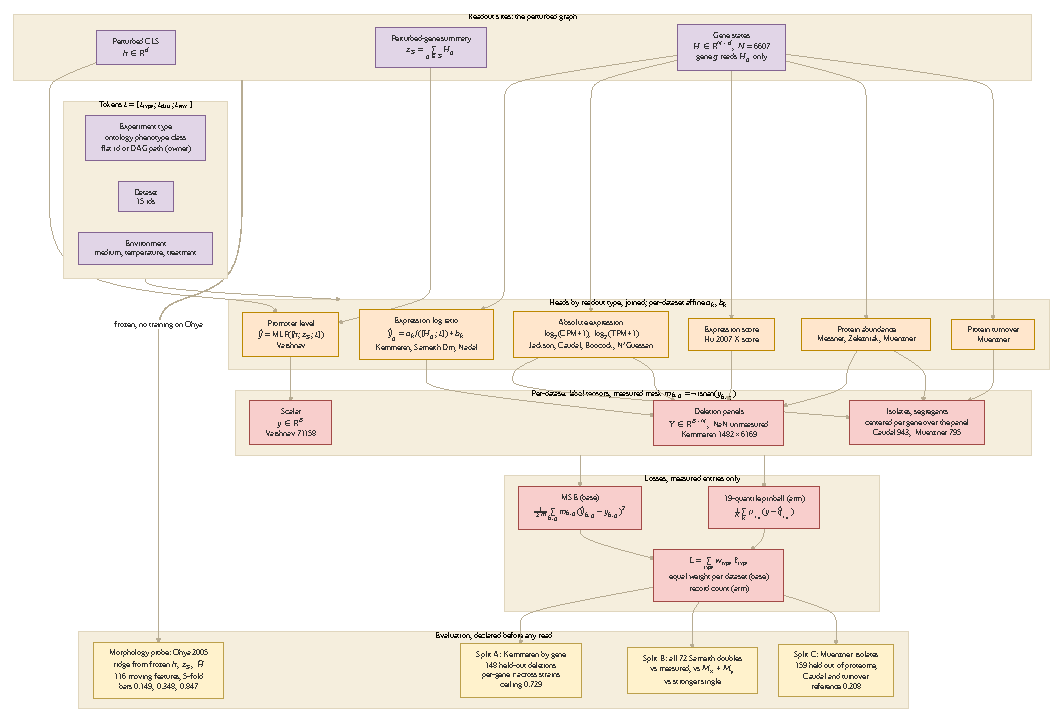
\includegraphics[width=0.92\linewidth]{figures/mermaid-output-side.pdf}\par\vspace{2pt}
\caption[]{\textbf{Gene-level readouts are read from each gene's own perturbed state
through heads joined by readout type, and Ohya is read only from the frozen latent.} Top,
the three readout sites of the perturbed graph; left, the experiment-type, dataset and
environment tokens; middle, the six heads with their per-dataset affines; then the label
tensors with their measured mask and the losses over measured entries; bottom, the
morphology probe and the three held-out splits. Placed on a rotated page at 241 mm,
a scale of 1.14 of the 212 mm rendering.}
\label{fig:output-side}
\end{figure}
\end{landscape}
%% Generated by notes/assets/publish/scripts/mermaid_pdf.sh from
%% notes/experiments.043-expression-proteome-morphology.mermaid.output-side.md

\subsection{Readout sites and the per-gene readout\secstatus{todo}}
\label{sec:output-sites}

The trunk returns three tensors per record after the perturbation operator: the perturbed
class token $h \in \mathbb{R}^d$, the perturbed gene states $H \in \mathbb{R}^{N \times d}$
over the $N = 6{,}607$ gene nodes, and the summary $z_S$. A gene-level value for gene $g$
is read from that gene's own state,
\begin{equation}
\hat y_{g} = a_{k}\, f_\theta\!\big([\,H_g \,;\, t\,]\big) + b_{k},
\qquad t = [\,t_{\mathrm{type}} \,;\, t_{\mathrm{data}} \,;\, t_{\mathrm{env}}\,],
\label{eq:pergene}
\end{equation}
with $f_\theta$ one head shared by every gene and every dataset of the readout type, $t$
the record's tokens (Sec.~\ref{sec:output-tokens}) and $(a_k, b_k)$ the affine of dataset
$k$. The prediction for gene $g$ depends on $H_g$ and on nothing else of $H$; the strain
reaches it through the trunk's attention and the perturbation operator, which is what
``from the node itself'' means in the equation. Four forms of $f_\theta$ are on the table.

\begin{itemize}
\item \textbf{Shared affine.} $f_\theta(x) = w^\top x + c$. The 019 head round measured
the linear per-gene readout within noise of the two-layer one on Kemmeren expression
($+0.002$ over four seeds, \texttt{H\_linear} against \texttt{H\_ref},
\texttt{2-readouts.tex}), so the nonlinearity is not known to carry anything there.
\item \textbf{Shared MLP with per-dataset affine} (Eq.~\ref{eq:pergene}; the prototype
\texttt{PerGeneReadout}). The affine is where the datasets' scales part.
\item \textbf{Shared MLP with the strain vector concatenated.} 019's \texttt{H\_concat}
feeds $[H_g ; c]$ with $c$ the strain context, and was the one arm above the reference in
every seed, $+0.0135$ with a seed sd of $0.0026$ on the difference (\texttt{2-readouts.tex},
Table \texttt{tab:readouts-head}). In Eq.~\ref{eq:pergene} this is $t$ extended by $z_S$.
\item \textbf{Cross-attention head.} One learned query per output feature over every token
(019 \texttt{M\_xattn}). On morphology it escaped under the pinball (4 of 4, $0.121 \pm
0.029$) and not under MSE (1 of 4) (\texttt{11-inductive.tex}). It reads the whole token
set, so it is not a readout from the node itself; it is the alternative if the per-gene
form stalls.
\end{itemize}

A record-level value (Vaishnav 2022, one level per promoter insert) is read from
$[h ; z_S ; t]$ through an MLP, the \texttt{GlobalHead} with \texttt{use\_pert\_summary}
that gave the 019 morphology result (12 of 12 escapes with MSE, $0.149 \pm 0.022$ over the
registered window, \texttt{11-inductive.tex}). The plain CLS escaped 0 of 8 under MSE at
two learning rates, so $h$ alone is not a readout site this design uses for a trained
target; it remains a probe input (Sec.~\ref{sec:output-protocol}).

\subsection{Joined or split heads\secstatus{todo}}
\label{sec:output-heads}

Two facts bound the choice. First, the datasets report different quantities on different
scales (Table~\ref{tab:output-scales}): a two-color $\log_2$ ratio to a wild-type pool, an
error-model X score, a pseudobulk $\log_2$ fold change with sentinels at $\pm 23$ to
$\pm 33$ in 20.2\% of cells (028, \texttt{2-readouts.tex}), UMI counts, TPM, a linear
MaxLFQ abundance, a log SWATH signal, a degradation rate per hour, a sort-seq bin level.
Second, datasets of one quantity agree weakly where they share a genotype
(Table~\ref{tab:cross}): Kemmeren against Hu 0.107, against Jackson 0.043 to 0.076,
against Nadal-Ribelles 0.002 per genotype; Messner against Zelezniak 0.049; Kemmeren mRNA
against Messner protein 0.031. An affine map preserves Pearson, so a per-dataset affine can
reconcile the first fact and cannot reconcile the second: a head shared by two datasets
that agree at 0.002 is asked to emit two unrelated vectors from the same $H_g$, told apart
only by the tokens.

\notesec{Joined by readout type}
Six heads (expression log ratio; absolute expression; expression score; protein abundance;
protein turnover; promoter level), each with one affine per dataset, 15 affines in all. The
datasets that would share a head and the agreement that supports it: Kemmeren and Sameith
Dm (the same arrays and procedures; Sameith's Methods defer to Kemmeren,
Sec.~\ref{sec:between}; the Kemmeren ceiling 0.729 is the only within-type ceiling) and,
under the same head by scale alone, Nadal-Ribelles at 0.002; Jackson, Boocock, N'Guessan
and Caudal under absolute expression (no shared genotype among them; Boocock and N'Guessan
share no segregant, Sec.~\ref{sec:within}); Messner, Zelezniak and Muenzner under protein
abundance (Messner against Zelezniak 0.049; Muenzner shares no genotype with either).
What a joined head buys is the transfer of the readout function across datasets, which is
the premise of the exercise and is unmeasured; what it risks is that a large low-agreement
dataset pulls the shared function away from the one with a ceiling.

\notesec{Split by dataset}
Fifteen heads, no sharing below the trunk. Datasets then meet only in $H$, which is what
every 019 round did with two array datasets (Kemmeren and Sameith) that are the same
arrays. Nothing is known about the trunk's transfer between readout types from this
campaign: proteome from genotype reached $0.085 \pm 0.008$ (v16, 12 runs) and expression
$0.180 \pm 0.006$ (v12, 4 runs) in separate trainings (\texttt{10-data-review.tex}); a joint
training of both was not scored on both.

\notesec{The proposal}
Joined by type with per-dataset affines, under the dataset token, with the two
low-agreement expression datasets (Nadal-Ribelles, Jackson) and Hu switched out as an
arm (Sec.~\ref{sec:output-protocol}). The split design is the control arm of the same
round, not a later step; the paired difference on the Kemmeren held-out score is the
answer. Hypothesis, untested: the affine will absorb the scale and the dataset token will
absorb the dataset's mean profile, leaving the shared head the per-gene response, which is
what transfers.

%% SOURCE: the released-quantity and transform columns are the 043 cross-dataset analysis
%% (notes/experiments.043-expression-proteome-morphology.md, "What each dataset reports");
%% the Nadal sentinel and Vaishnav rows are this section's proposal.
\begin{table}[htbp]
\centering
\scriptsize
\setlength{\tabcolsep}{3pt}
\caption[]{\textbf{Readout type and target transform per dataset.} The transform column is
what the loss sees; ``as released'' means the stored value. The transforms for Jackson,
Caudal, Messner, Zelezniak and Muenzner are the ones the cross-dataset analysis used
(Table~\ref{tab:cross}); the Nadal-Ribelles and Vaishnav rows are proposals.}
\label{tab:output-scales}
\begin{tabular}{>{\raggedright\arraybackslash}p{30mm}>{\raggedright\arraybackslash}p{30mm}>{\raggedright\arraybackslash}p{46mm}>{\raggedright\arraybackslash}p{62mm}}
\toprule
Dataset & Readout type (head) & Released quantity, scale & Target transform \\
\midrule
Kemmeren 2014; Sameith 2015 Dm & expression log ratio & two-color array, $\log_2$ (deletion / WT pool) & as released \\
Nadal-Ribelles 2025 & expression log ratio & pseudobulk $\log_2$ fold change vs WT & as released, with $|{\cdot}| > 20$ set to missing (the zero-mean sentinel; 20.2\% of cells) \\
Hu 2007 & expression score & error-model X score vs BY4741, signed & as released; its own head, since an X score is not a log ratio \\
Jackson 2020 & absolute expression & pseudobulk UMI counts, zeros omitted & $\log_2((\mathrm{CPM}+1)/(\mathrm{CPM}_{\mathrm{HO}}+1))$ against the HO deletion of the same environment, or $\log_2(\mathrm{CPM}+1)$ with the environment token carrying the condition (owner decision) \\
Boocock 2025; N'Guessan 2025 & absolute expression & UMI counts per segregant & $\log_2(\mathrm{CPM}+1)$, centered per gene within the panel \\
Caudal 2024 & absolute expression & RNA-seq TPM, linear & $\log_2(\mathrm{TPM}+1)$, centered per gene over the isolates \\
Messner 2023 & protein abundance & SWATH MaxLFQ, linear & $\log_2$(strain / record reference) \\
Zelezniak 2018 & protein abundance & SWATH log signal (SVA) & strain minus record reference \\
Muenzner 2024 protein & protein abundance & SWATH MaxLFQ precursor quantity, linear & $\log_2$, centered per protein over the isolates \\
Muenzner 2024 turnover & protein turnover & dynamic SILAC degradation rate, per hour & $\log_2$, centered per protein over the isolates \\
Vaishnav 2022 & promoter level & sort-seq expression level, one scalar & standardized over the library \\
\bottomrule
\end{tabular}
\end{table}

\subsection{The experiment-type, dataset and environment tokens\secstatus{todo}}
\label{sec:output-tokens}

Three learned vectors travel with every record. The \textbf{experiment-type token} is the
record's ontology phenotype class: \texttt{Microarray\allowbreak Expression\allowbreak Phenotype} (Kemmeren,
Sameith), \texttt{Microarray\allowbreak Expression\allowbreak Score\allowbreak Phenotype} (Hu),
\texttt{Single\allowbreak Cell\allowbreak Expression\allowbreak Phenotype} (Jackson, Boocock, N'Guessan),
\texttt{Pseudobulk\allowbreak Expression\allowbreak Phenotype} (Nadal-Ribelles), \texttt{RNASeq\allowbreak Expression\allowbreak Phenotype}
(Caudal), \texttt{Protein\allowbreak Abundance\allowbreak Phenotype} (Messner, Zelezniak, Muenzner),
\texttt{Protein\allowbreak Turnover\allowbreak Phenotype} (Muenzner) and \texttt{Pooled\allowbreak Sort\allowbreak Seq\allowbreak Expression\allowbreak Phenotype}
(Vaishnav), the classes of Table~\ref{tab:store}'s rows. The \textbf{dataset token} is the
dataset's id. The \textbf{environment token} is the record's medium, temperature and
environmental perturbation, which separates Jackson's eleven conditions and Nadal-Ribelles'
two.

\notesec{The precedent}
Experiment 035 gave the cell graph transformer a compound token $z_E$ from a fingerprint
MLP and asked whether it predicts Vanacloig 2022 for an unseen compound. Three entry points
were measured on 123 compound-evaluations (\texttt{experiments.035}, rounds 9 and 10): a
bilinear factor at the head ($-0.007$ paired against ridge, 95\% CI $-0.028$ to $+0.015$),
a gate on every gene's state ($-0.025$), and a token the genes attend to for one further
layer ($+0.008$, CI $-0.026$ to $+0.045$; $+0.015$ against the head form, CI through zero).
The ablation was the arm with no compound input (\texttt{cgt\_genes}), whose centered score
is zero by construction. The same three entry points and the same ablation apply here.

\notesec{Where the tokens enter}
(i) At the head only: $t$ concatenated to $H_g$ in Eq.~\ref{eq:pergene} and to $[h ; z_S]$
for the record-level head. Cheapest, and the 035 bilinear form's analog. (ii) On the CLS
row: $t$ added to the class token before the trunk, so every gene can attend to it. (iii)
As a token the genes attend to in one further layer after the perturbation operator, the
035 environment-encoder form, the only one of the three with a positive paired mean
against ridge there. The ablation arm carries no token, and a second ablation carries the
dataset token only, which says whether the experiment type adds anything over the dataset
id (hypothesis, untested: with 15 datasets and 8 classes the two are nearly collinear, and
the type token earns its place only on a dataset unseen in training).

\notesec{Flat id or ontology path}
A flat token is one row per class. A path token sums one row per node of the class's
ontology path, so \texttt{MicroarrayExpressionPhenotype} and
\texttt{RNASeqExpressionPhenotype} share an expression row and differ in their own
(prototype \texttt{ExperimentTypeEmbedding}, \texttt{mode="dag"}). The fact that decides
it: the served graph has no such path. Every phenotype class is a direct child of
\texttt{phenotype} in \texttt{biocypher/config/torchcell\_schema\_config.yaml} (the
\texttt{phenotype member of} edge lists all 34 leaves), and in the pydantic schema only
the two microarray classes share a parent below \texttt{Phenotype}
(\texttt{TwoChannelMicroarrayExpressionPhenotype}). A path token therefore needs a
grouping written on the modeling side (expression, protein, morphology, promoter), or it
waits for the ontology unification to supply one. That is an owner decision
(Sec.~\ref{sec:output-decisions}); the flat token needs nothing new.

\subsection{Losses\secstatus{todo}}
\label{sec:output-losses}

Each readout type has one loss over the measured entries of its records only: a missing
gene is \texttt{NaN} in the target tensor, contributes no value and no gradient, and a type
with nothing measured in a batch returns a connected zero (prototype
\texttt{MaskedTypedLoss}, the convention of \texttt{masked\_mean} in
\texttt{torchcell/losses/distributional.py}). Three choices remain.

\notesec{MSE or pinball}
019 trained expression with the 19-quantile pinball and read the median; on morphology, MSE
on \texttt{M\_zs} escaped 12 of 12 runs by epoch 410 with the smallest spread of any cell,
the pinball on the same readout 8 of 10 and late (epochs 230 to 770), and MSE on the CLS 0
of 8 (\texttt{11-inductive.tex}). The loss and the readout interact, so neither is chosen
for the per-gene heads by that result; the design runs MSE as the default and the pinball
as an arm, both on the per-gene form. The Pearson loss and ListMLE are not arms: five of
six batch-32 Pearson runs collapsed to a constant output and the anchored ListMLE runs sat
on the mean by epoch 250 (\texttt{2-readouts.tex}).

\notesec{Weighting across datasets}
By record the store is 173{,}617 samples, of which Boocock holds 79{,}516 and Vaishnav
71{,}158 (Table~\ref{tab:store}), 87\% of the records in two datasets with no gene-level
deletion genotype; Kemmeren is 1{,}482. A loss averaged over measured entries weights
datasets by records times features, so the deletion panels would be a few percent of the
gradient. Three rules: equal weight per dataset (each dataset's mean loss summed); weight
by the ceiling, so Kemmeren (0.729), Messner (0.696) and Zelezniak (0.916) count more
than Nadal-Ribelles (0.043 against 0.022 across batches) and Jackson (0.129 against
0.095); or by record count. The proposal is equal weight per dataset with the
low-agreement datasets down-weighted by their agreement, and the record-count rule as
the arm that shows what the segregant panels do to the deletion score.

\notesec{Scale}
Every linear quantity is logged before the loss (Table~\ref{tab:output-scales}); every
pair in Table~\ref{tab:cross} was compared log against log, and a correlation does not
depend on the base. Centering per gene over a panel (Caudal, Muenzner, the segregants) is
what the cross-dataset analysis did and is the only way those panels have a zero; it means
their head predicts a deviation from the panel mean, the same object a deletion dataset's
log ratio is.

\subsection{The evaluation protocol\secstatus{todo}}
\label{sec:output-protocol}

Three held-out sets, one probe, four arms and a scoring rule, declared before any run is
read (Table~\ref{tab:output-protocol}).

\notesec{Split A, Kemmeren by gene}
A fraction of Kemmeren's 1{,}482 deletion genotypes, 10\% or 148 genes, is held out by
gene: no record in any deletion dataset whose perturbation set contains a held-out gene is
trained on (Kemmeren, Hu, Jackson, Nadal-Ribelles, Messner, Zelezniak, Ohya), so the gene
is unseen as a perturbation on any readout. A held-out gene still appears in the isolates
and segregants as a sequence variant, an absence or an inherited block; those are not
deletions and are not held out, and an arm without the natural-genome datasets
(below) measures what that leakage, if it is one, is worth. The score is the per-gene
Pearson across the 148 held-out strains for each of the 6{,}169 genes (mean and median
over genes) and the per-strain Pearson across genes (median over strains), both against
the own-culture ceiling 0.729 (test-retest, 114 mutants) and 0.653 (decomposition,
Table~\ref{tab:kemmeren}). The 019 reference on Kemmeren plus Sameith is $0.180 \pm
0.006$ per gene over four runs and 0.233 for one 10{,}000-epoch run
(\texttt{10-data-review.tex}); the 019 split was by strain with the same gene set, so it
is a reference and not a paired bar. The Sameith Sm records are excluded from the store's
training set outright: they are Kemmeren's arrays (82 of 82 identical).

\notesec{Split B, every Sameith double}
All 72 Sameith 2015 double deletions are held out; their constituent singles (82
distinct deletions, the Sameith Sm set) are in training as Kemmeren profiles, so the task
is inference into the combinatorial space from measured singles. Each double is scored against its measured profile (per-strain Pearson
over 6{,}169 genes; per-gene Pearson across the 72 doubles) and paired against two nulls
that need no model: the additive null $M_x + M_y$ from the two Kemmeren singles, which is
the paper's own expected value (``the deviation between the expression change observed in
the double mutant $M_{x\Delta y\Delta i}$ and the expected expression change, given each
single mutant $M_{x\Delta i} + M_{y\Delta i}$'', paper.md line 39), and the stronger
single alone. A third score restricts the genes to those where the double departs from the
additive null by more than the paper's threshold, $|M_{xy,i} - (M_{x,i} + M_{y,i})| >
\log_2 1.5$: on those genes the additive null is wrong by construction and the question is
whether the model is less wrong. Sameith ran ``four times from two independent cultures''
per mutant (paper.md line 33) and released one profile, so no double has a ceiling of its
own; the Kemmeren 0.729 is the bound for the same arrays and procedures.

\notesec{Split C, Muenzner isolates}
A fifth of the 795 Muenzner 2024 proteome isolates, 159, is held out by isolate, and the
same isolates are held out from Caudal 2024 (759 shared) and from the turnover set (55
isolates), so a held-out strain is unseen on every readout. The score is the per-protein
Pearson across the held-out isolates over 1{,}540 proteins and the per-isolate Pearson
across proteins. No Muenzner replicate ceiling is measured (Table~\ref{tab:store}); the
Caudal against Muenzner agreement, 0.208 per isolate and 0.160 per gene
(Table~\ref{tab:cross}), is the reference for what another readout of the same strain
reaches, and the 019 proteome-from-genotype reading on Messner deletions, $0.085 \pm
0.008$, is the reference for the deletion head. Whether an isolate can enter the trunk at
all is the input-side design's question; split C is declared so that the answer has a
test ready.

\notesec{The morphology probe}
Ohya 2005 enters no training. For each of its 4{,}678 genotypes the frozen model produces
$h$, $z_S$ and the mean over genes of $H$; a ridge from each, and from their
concatenation, to the 116 moving CalMorph features is fit 5-fold over genotypes with the
penalty chosen on an inner split, inputs and targets z-scored and clipped at 8, and
scored as the out-of-fold Pearson per feature across held-out genotypes, median over the
116 (the construction of Table~\ref{tab:morph}). The bars, in order: the 019 genotype-only
model read through its own trained head, $0.149 \pm 0.022$; the sequence-embedding ridge
0.08 to 0.14 (\texttt{11-inductive.tex}); the Kemmeren-expression ridge 0.348 on the
1{,}437 shared genotypes and the Messner ridge 0.278 on 4{,}279 (Table~\ref{tab:morph}),
which read the strain's own measurement and are the transductive bars; and the ceiling
0.847 on the 116 features (019) or 0.611 over the 281 (122 wild-type replicates,
Table~\ref{tab:store}). A probe at or above 0.348 from the genotype alone would say the
latent carries what the measured expression carries; one near 0.149 says the probe is the
trained head by another route.

\notesec{Arms}
Four arms in a $2 \times 2$: with and without the natural-genome datasets (Caudal,
Muenzner protein and turnover, Boocock, N'Guessan), with and without Vaishnav; plus the
split-head control and the no-token ablation on the full arm, and the deletion-only
reference (Kemmeren and Messner; Sameith Dm is split B and does not train). Every arm is scored on
splits A, B and the probe; split C exists only in the arms that train isolates. Three
initializations and two split seeds per arm, as 019's v25 (four split seeds, three
initializations) found the escape to be a property of the run and not the split.

\notesec{Window and reads}
The epoch budget and the window are declared with the launch; 019's rule was 500 epochs
read over epochs 400 to 499, declared 2026-10-12, and its 1{,}000-epoch runs scored lower
over 900 to 999 than over 400 to 499 in 7 of 8. A cell is read first by its escape
fraction and second by its window mean; no maximum over epochs is reported. The test
indices of every split are pinned to a file before training and the split-B and split-C
scores are read once, at the end of the round.

%% SOURCE: the n, bar and metric columns cite notes/experiments.043-expression-proteome-morphology.md
%% (store table, cross-dataset and within-dataset sections) and the 019 retrospective.
\begin{table}[htbp]
\centering
\scriptsize
\setlength{\tabcolsep}{3pt}
\caption[]{\textbf{The evaluation protocol.} Every bar is a measured number; a reference is
a number from a different split or model and is marked so.}
\label{tab:output-protocol}
\begin{tabular}{>{\raggedright\arraybackslash}p{18mm}>{\raggedright\arraybackslash}p{44mm}>{\raggedright\arraybackslash}p{22mm}>{\raggedright\arraybackslash}p{44mm}>{\raggedright\arraybackslash}p{42mm}}
\toprule
Split & Held out & n & Metric & Bar \\
\midrule
A, Kemmeren by gene & 10\% of Kemmeren deletion genes; every deletion record naming one, in every deletion dataset & 148 strains, 6{,}169 genes & per-gene Pearson across held-out strains (mean, median over genes); per-strain Pearson across genes (median) & ceiling 0.729 test-retest, 0.653 decomposition; reference 019 by-strain $0.180 \pm 0.006$ \\
B, Sameith doubles & all 72 double deletions; the 82 constituent singles stay in training as Kemmeren records & 72 strains, 6{,}169 genes & per-strain Pearson vs measured; paired difference vs the additive null $M_x + M_y$ and vs the stronger single; the same on genes with $|M_{xy} - (M_x + M_y)| > \log_2 1.5$ & additive null (no model); ceiling 0.729 (same arrays, no double replicate) \\
C, Muenzner isolates & a fifth of the proteome isolates, the same strains out of Caudal and turnover & 159 isolates, 1{,}540 proteins (turnover: those of its 55 among them) & per-protein Pearson across held-out isolates; per-isolate Pearson across proteins & no Muenzner ceiling measured; reference Caudal $\times$ Muenzner 0.208 per isolate, 0.160 per gene; reference 019 Messner $0.085 \pm 0.008$ \\
Morphology probe & Ohya 2005, never trained; 5-fold over genotypes & 4{,}678 genotypes, 116 moving features & ridge from frozen $h$, $z_S$, $\bar H$, their concatenation; out-of-fold Pearson per feature, median over 116 & 019 trained head $0.149 \pm 0.022$; sequence ridge 0.08 to 0.14; Kemmeren ridge 0.348 (1{,}437), Messner 0.278 (4{,}279), transductive; ceiling 0.847 (116) or 0.611 (281) \\
\bottomrule
\end{tabular}
\end{table}

\subsection{Owner decisions\secstatus{todo}}
\label{sec:output-decisions}

\begin{enumerate}
\item \textbf{Joined or split heads.} Joined by readout type with per-dataset affines (six
heads, 15 affines), or one head per dataset (15 heads). Facts: same-type agreement is
0.002 to 0.107 for expression and 0.049 for protein (Table~\ref{tab:cross}); an affine
cannot raise a correlation; no joint training across types has been scored. Proposal:
joined, with split as the control arm.
\item \textbf{Flat or path token for the experiment type.} The served ontology is flat
(34 leaves under \texttt{phenotype}); a path needs a modeling-side grouping or the
unification. Proposal: flat now, path when the ontology carries one.
\item \textbf{Where the tokens enter.} Head only, CLS row, or attended token (035's three
forms; $-0.007$, $-0.025$, $+0.008$ against ridge, all CIs through zero). Proposal: head
only as the base, attended token as the arm.
\item \textbf{Loss.} MSE or the 19-quantile pinball on the per-gene heads (019: MSE on
$z_S$ 12 of 12 escapes, pinball 8 of 10, on morphology only). Proposal: MSE base, pinball
arm.
\item \textbf{Dataset weighting.} Equal per dataset, by ceiling, or by record count (two
datasets hold 87\% of the records). Proposal: equal per dataset, agreement-weighted for
the low-agreement sets, record count as an arm.
\item \textbf{Nadal-Ribelles sentinels.} Treat $|\log_2 \mathrm{FC}| > 20$ as missing
(20.2\% of cells), or keep the stored value. Proposal: missing.
\item \textbf{Jackson target.} Deletion effect against the HO control of the same
environment, or the absolute $\log_2(\mathrm{CPM}+1)$ with the environment token carrying
the condition. Facts: construction pairs agree at 0.129 against 0.095 on the effect, and
one genotype across environments at 0.010. Proposal: the effect.
\item \textbf{Split A leakage rule.} Hold the gene out of every deletion dataset (proposed)
or out of the expression datasets only; the natural-genome arm measures the isolate and
segregant side either way.
\item \textbf{Split C size and existence.} A fifth of the isolates held out, contingent on
the input-side design admitting isolates at all.
\item \textbf{Budget and window.} Epochs and window to declare with the launch; 019's 500
and 400 to 499 are the precedent.
\end{enumerate}
